\documentclass{article}
%% PACKAGES %%

\usepackage{amsmath, amsfonts, amssymb, amsthm}
\usepackage{braket}
\usepackage{listings}
\usepackage{geometry}
\usepackage{xcolor}
\usepackage{textcomp}
\usepackage{graphicx}
\usepackage{fancyhdr}
\usepackage{sourcecodepro}
\usepackage{multirow}

%%%%%%%%%%%%%%

\graphicspath{{./images}}
\setlength\parindent{0pt}       % globally supress indentation

%% LISTINGS CONFIG %%

\definecolor{purple2}{RGB}{153,0,153} % there's actually no standard purple
\definecolor{green2}{RGB}{0,153,0} % a darker green

\lstset{
  language=MATLAB,                   % the language
  basicstyle=\normalsize\ttfamily,   % size of the fonts for the code
  frame = single,
  % Color settings to match IDLE style
  keywordstyle=\color{orange},       % core keywords
  keywordstyle={[2]\color{purple2}}, % built-ins
  stringstyle=\color{green2},%
  showstringspaces=false,
  commentstyle=\color{red},%
  upquote=true,                      % requires textcomp
  numbers=left,
  breaklines=true,
}

% Title Stuff
\title{\vspace{-3cm}ECE355L Task 5 \\ Convolution of Signals}
\author{Chase A. Lotito, \textit{SIUC Undergraduate}}
\date{}

\begin{document}

\pagestyle{fancy}

% attempt to make nice header
\fancyhead{}
\fancyhead[CH]{\normalsize{LOTITO --- ECE355L --- TASK 5}}

\maketitle % Makes the title

\section*{Part I: Convolution Calculations}

\subsection*{Exercise 1}

Plot the respective graphs for the above examples and include in the report.

\smallskip

\textbf{Solution.}

\smallskip

All I did was copy the code from the lab manual, and after running those MATLAB scripts, I get the following plots:

\begin{figure}[!ht] 
    \centering
    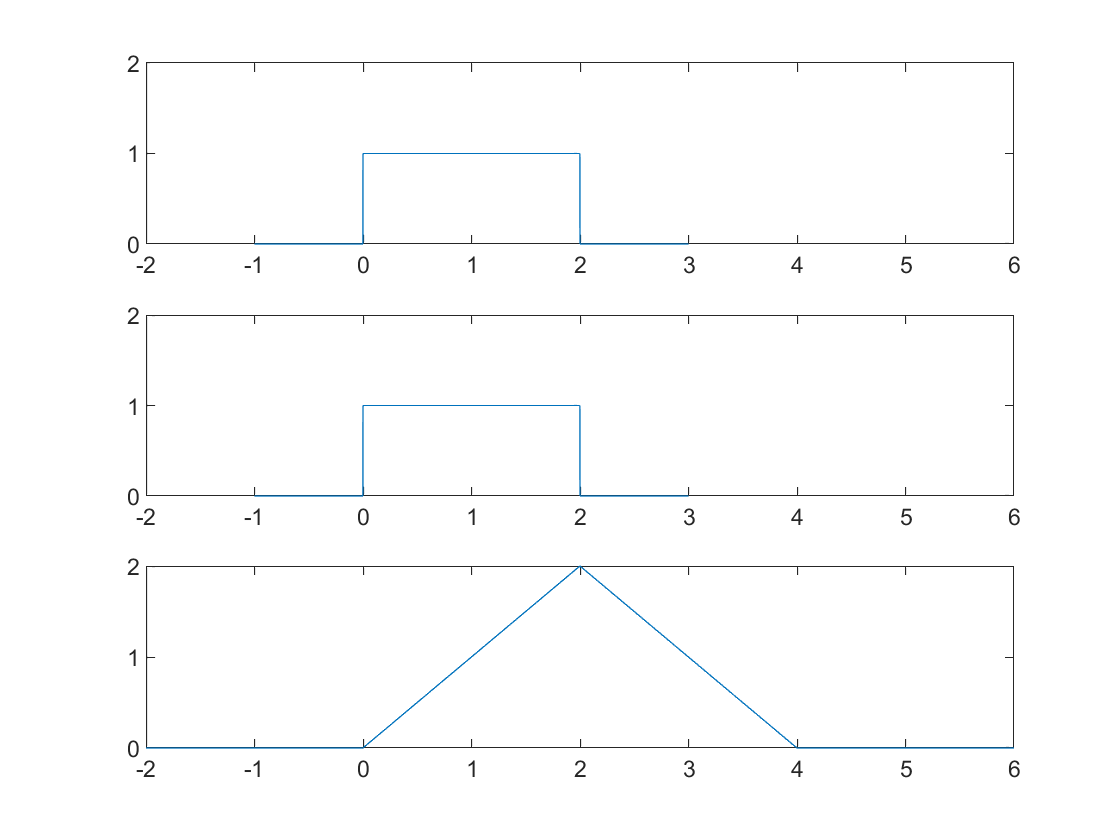
\includegraphics[width = 7cm]{plot1.png}
    \caption{Example 1 Plot}
    \label{fig:firstplot}
\end{figure}

\begin{figure}[!ht] 
    \centering
    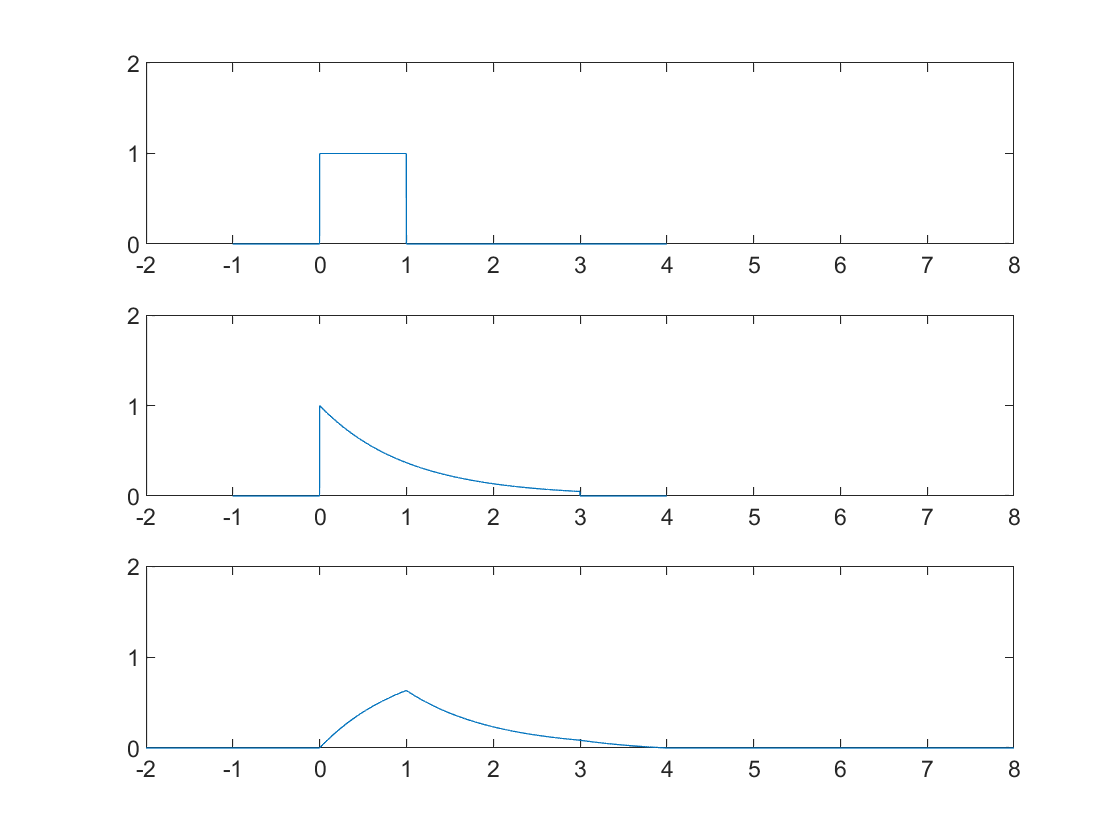
\includegraphics[width = 7cm]{plot2.png}
    \caption{Example 2 Plot}
    \label{fig:secondplot}
\end{figure}

\clearpage

\subsection*{Exercise 2}

Plot the following signals on the same window, but separate graphs using the subplot command and axis so that all graphs have the same range for the time (as was done in the examples). Let \(-2 \leq t \leq 25\) with a step size of 0.001 for \(f(t)\) and \(g(t)\). The convolution, \(y(t)\), product will then be evaluated for \(-4 \leq t \leq 50\).

\begin{equation*}
    \begin{gathered}
        f(t) = \sin \left( \frac{\pi}{10} t \right) \times [u(t) - u(t-20)] \\
        g(t) = \cos \left( \frac{\pi}{5} t \right) \times [u(t) - u(t-15)]  \\
        y(t) = f(t) * g(t)
    \end{gathered}
\end{equation*}

\smallskip

\textbf{Solution.}

\smallskip

To convolve \(f\) and \(g\) and then plot them with \(y\), I wrote the following MATLAB code:

\begin{lstlisting}
% Chase Lotito - ECE355L - Project 3
% PART 1: Plotting Convolutions
% Question 2

dt = 0.001;     % step size
t = -2:dt:25;   % f and g interval
t_y = -4:dt:50; % convolution interval

f = sin(t * pi / 10) .* rectpuls((t-10), 20);
g = cos(t * pi / 5) .* rectpuls((t-7.5), 15);
y = dt*conv(f, g);

% Plot all the convolutions
subplot(3,1,1), plot(t,f), title('f(t)'), axis([-2 25 -2 2]);
subplot(3,1,2), plot(t,g), title('g(t)'), axis([-2 25 -2 2]);
subplot(3,1,3), plot(t_y,y, 'r'), title('y(t) = f(t) * g(t)'), axis([-4 50 -3 2]);
\end{lstlisting}

The output plot from the code is:

\begin{figure}[!ht] 
    \centering
    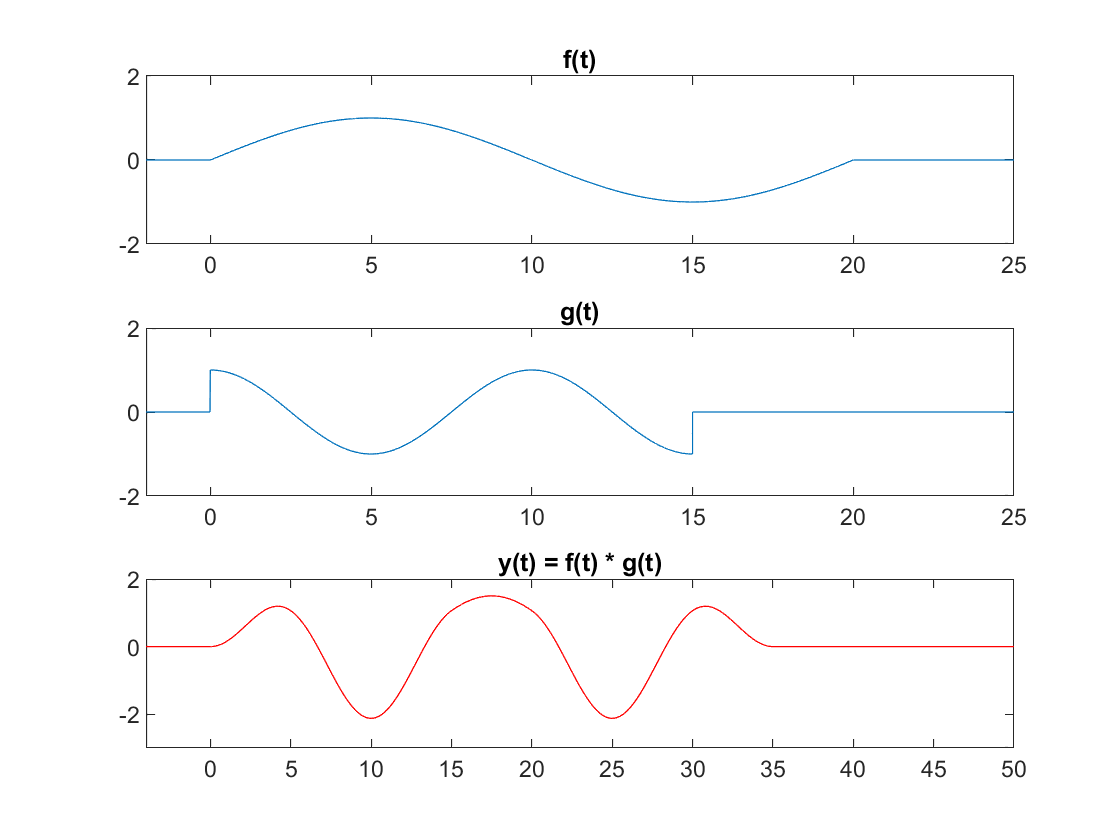
\includegraphics[width = 15cm]{plot3.png}
    \caption{\(f(t)\), \(g(t)\), and \(y(t)\)}
    \label{fig:thirdplot}
\end{figure}

\clearpage

\section*{Part II: Convolution Reverb}

Using the audio files provided on the D2L, we can use \textit{audioread()} to get an \((m \times n)\) matrix containing the audio data, where we have \(m\) samples, and \(n\) audio channels (2 for stereo). We also get a sampling rate \(fs=480000~s^{-1}\). We can listen to these audio files using \textit{sound()}.

\bigskip

To add reverb to \textit{"audio\_sample.wav"}, we need to convolve the impulse response of an environment with reverberation--like a large hall, and a small hall. By convolving the audio-sample with the impulse reponses, we will hear how the audio-sample would have sounded in each respective environment.  

\bigskip

Since the convolution function \textit{conv()} only takes vector inputs, we have to convert the stereo audio sample-data to mono. We can do this using \textit{mean(A,2)} for some matrix \(A\). The mean function will average each row and return a column vector containing these averages.

\begin{lstlisting}
% Chase Lotito - ECE355 Project 3 Part II

% Take audio inputs for: sample, large hall, and small hall
% audioread() returns --> [sample-data, sample-rate]
% sample-data is a (mxn) matrix, m-samples with n-audio-channels
[a,fs] = audioread('audio_sample.wav');
[h1,fs] = audioread('impulse_response1.wav'); % large hall
[h2,fs] = audioread('impulse_response2.wav'); % small hall

sound(a,fs);
pause(5);
sound(h1,fs);
pause(5);
sound(h2,fs);

% a, h1, and h2 are (mx2) matricies, since stereo audio,
% use mean(A,2) to average each row and return a column vector
% conv() only accepts vector inputs (or use conv2)
conv_rev1 = conv(mean(a,2),mean(h1,2));
pause(5);
sound(conv_rev1,fs);

conv_rev2 = conv(mean(a,2),mean(h2,2));
pause(5);
sound(conv_rev2,fs);

t1 = 0:1/fs:(length(a)/fs)-(1/fs);
t2a = 0:1/fs:(length(h1)/fs)-(1/fs);
t2b = 0:1/fs:(length(h2)/fs)-(1/fs);
t3a = 0:1/fs:((length(a)+length(h1)-1)/fs)-(1/fs);
t3b = 0:1/fs:((length(a)+length(h2)-1)/fs)-(1/fs);

subplot(2,3,1);
plot(t1,a),xlabel('Time(s)'),ylabel('Amplitude'),title('Original audio sample');
subplot(2,3,2)
plot(t2a,h1),xlabel('Time(s)'),ylabel('Amplitude'),title('Impulse response 1 (Large Room)')
subplot(2,3,3)
plot(t3a,conv_rev1), xlabel('Time(s)'),ylabel('Amplitude'),title('Convoluted audio sample for a large room')
subplot(2,3,4);
plot(t1,a),xlabel('Time(s)'),ylabel('Amplitude'),title('Original audio sample');
subplot(2,3,5)
plot(t2b,h2),xlabel('Time(s)'),ylabel('Amplitude'),title('Impulse response 2 (small Room)')
subplot(2,3,6)
plot(t3b,conv_rev2), xlabel('Time(s)'),ylabel('Amplitude'),title('Convoluted audio sample for a small room')
\end{lstlisting}

The new audio samples are now considerably louder, but each have reverb. The large-hall audio sample is louder and has a longer decay. The small-hall audio sample is quieter, more distinct, and decays faster.

\begin{figure}[!ht] 
    \centering
    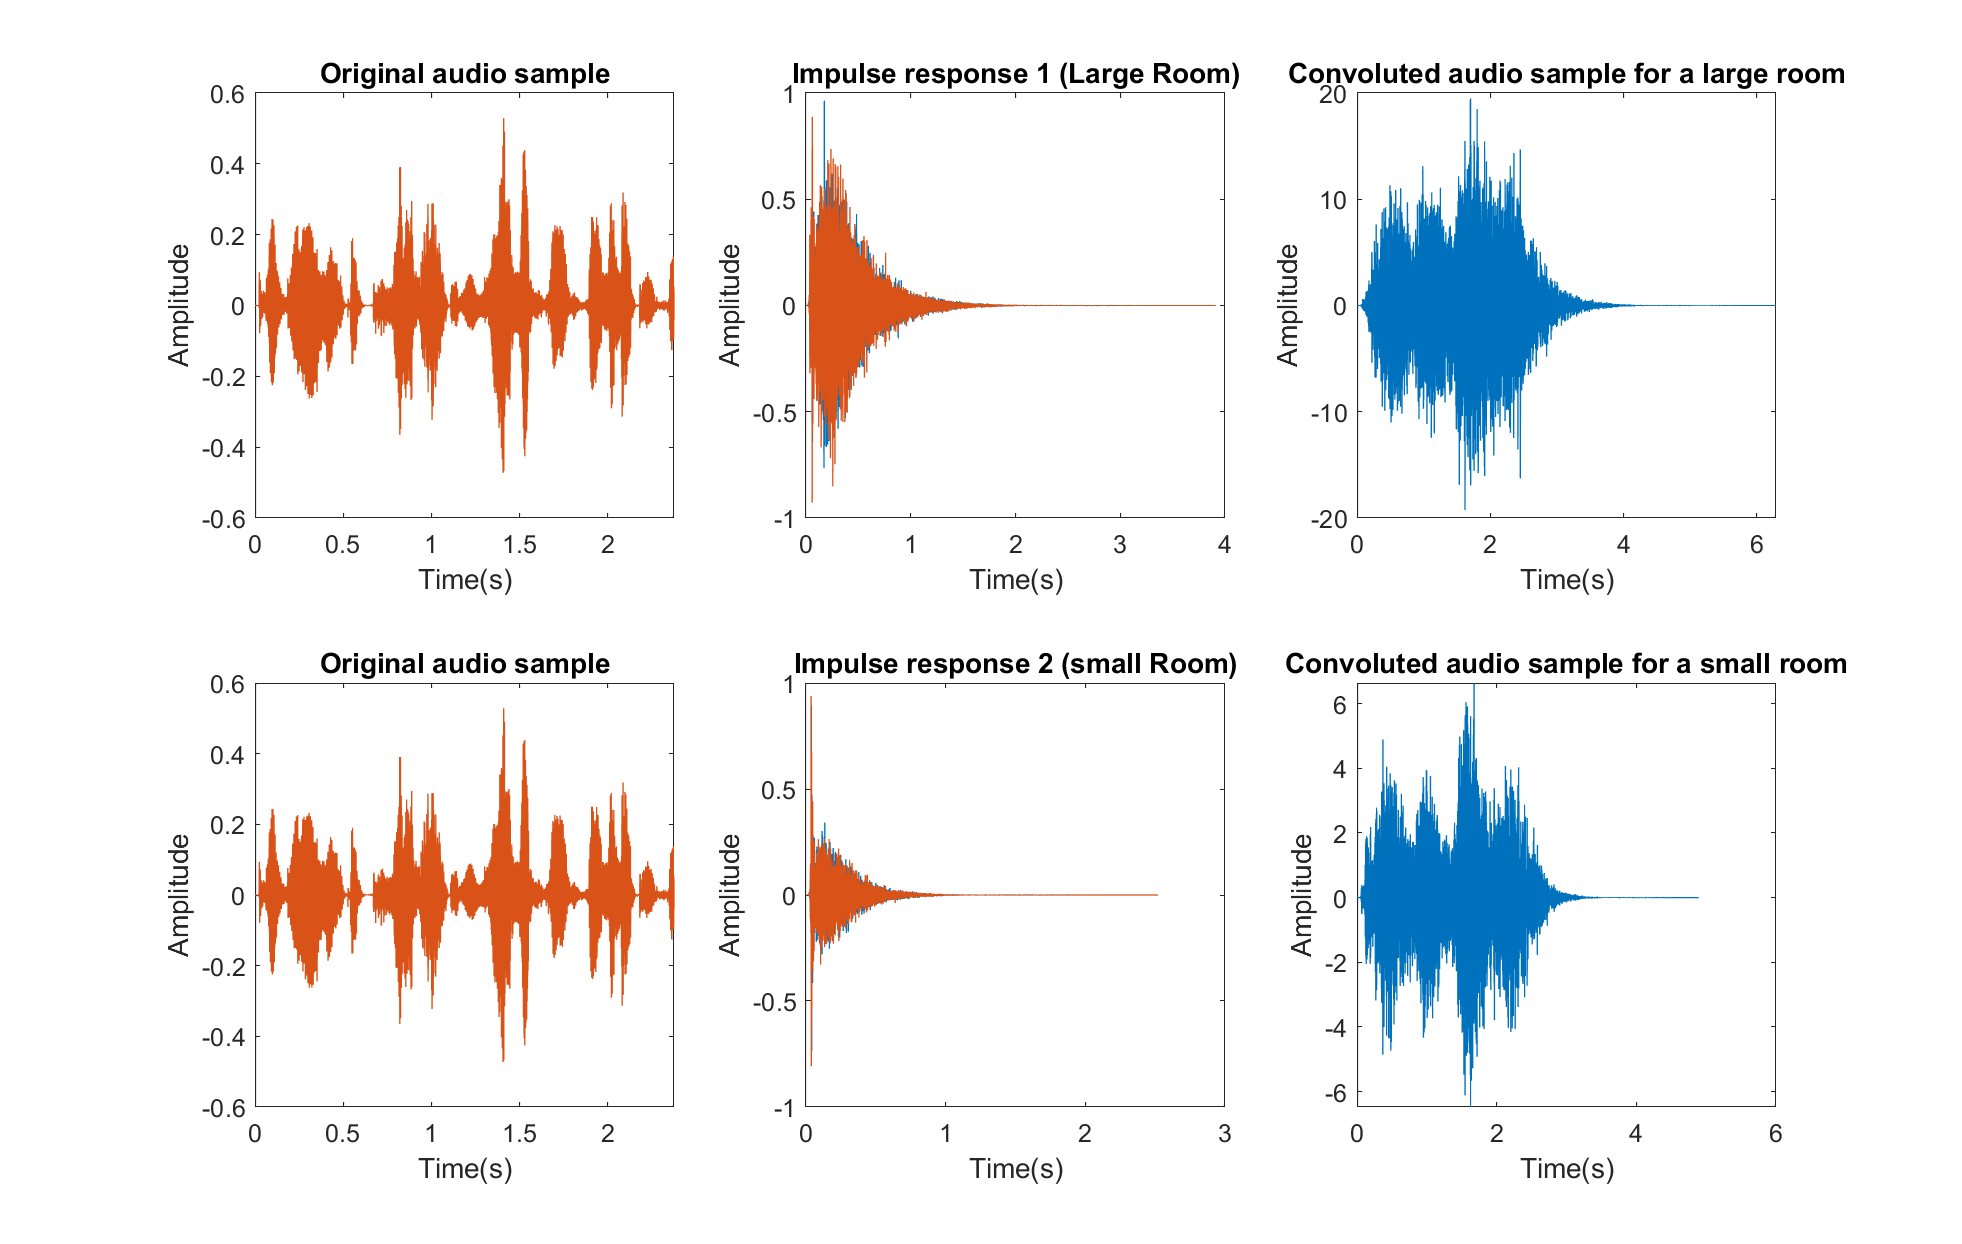
\includegraphics[width = 15cm]{audio-plot.png}
    \caption{Audio Plots: original, large hall, small hall.}
    \label{fig:audioplot}
\end{figure}


\end{document}
